Fill in the blanks to make true identities:
\begin{enumerate}[label=(\alph*)]
\item $(A \triangle B) \cap C = (C \setminus A) \triangle $ \makebox[1cm]{\hrulefill}.
\item $C \setminus (A \triangle B) = (A \cap C) \triangle $ \makebox[1cm]{\hrulefill}.
\item $(B \setminus A) \triangle C = (A \triangle C) \triangle $ \makebox[1cm]{\hrulefill}.
\end{enumerate}

\textbf{Solution:} 
\

\textbf{15(a)}: Consider that $(A \triangle B) \cap C = [(A \wedge C) \vee (B \wedge C)] \wedge \neg (A \wedge B)$. \\ The corresponding Venn diagram is shown below. \\
Note the symmetry, we guess that $(A \triangle B) \cap C = (C \setminus A) \triangle (C \setminus B)$.

\

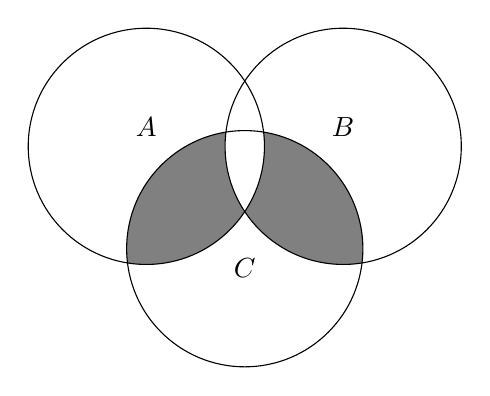
\begin{tikzpicture}
% Define circles for A, B, and C
\def\circleA{(-0.5,0) circle (1.5cm)}
\def\circleB{(2,0) circle (1.5cm)}
\def\circleC{(0.75,-1.3) circle (1.5cm)}

% Shade (A and C) excluding (A and B)
\begin{scope}
\clip \circleA;
\clip \circleC;
\fill[gray] \circleC;
\clip \circleB;
\fill[white] \circleB;
\end{scope}

% Shade (B and C) excluding (A and B)
\begin{scope}
\clip \circleB;
\clip \circleC;
\fill[gray] \circleC;
\clip \circleA;
\fill[white] \circleA;
\end{scope}

% Outline the circles and label them
\draw \circleA node [text=black, above] {$A$};
\draw \circleB node [text=black, above] {$B$};
\draw \circleC node [text=black, below] {$C$};
\end{tikzpicture}
\pagebreak

Below is the prove for \textbf{15(a)}. 
\begin{alignat*}{2}
&x \in (C \setminus A) \triangle (C \setminus B) && \quad \textbf{(1)}\\
&\equiv x \in [(C \setminus A) \cup (C \setminus B)] \setminus [(C \setminus A) \cap (C \setminus B)] && \quad \textbf{(2)}\\
&\equiv x \in [(C \setminus A) \cup (C \setminus B)] \setminus Q && \quad \textbf{(3)}\\
&\equiv [x \in (C \setminus A) \cup (C \setminus B)] \wedge \neg (x \in Q) && \quad \textbf{(4)}\\
&\equiv [x \in C \setminus A \vee x \in C \setminus B] \wedge \neg (x \in Q) && \quad \textbf{(5)}\\
&\equiv \{[x \in C \wedge \neg (x \in A)] \vee [x \in C \wedge \neg (x \in B)]\} \wedge \neg (x \in Q) && \quad \textbf{(6)}\\
&\equiv \{([x \in C \wedge \neg (x \in A)] \vee x \in C) \wedge ([x \in C \wedge \neg (x \in A)] \vee \neg [x \in B])\} \wedge \neg (x \in Q) && \quad \textbf{(7)}\\
&\equiv \{(x \in C) \wedge ([x \in C \wedge \neg (x \in A)] \vee \neg [x \in B])\} \wedge \neg (x \in Q) && \quad \textbf{(8)}\\
&\equiv \{(x \in C \wedge [x \in C \wedge \neg (x \in A)]) \vee [x \in C \wedge \neg (x \in B)]\} \wedge \neg (x \in Q) && \quad \textbf{(9)}\\
&\equiv \{([x \in C \wedge x \in C] \wedge \neg (x \in A)) \vee [x \in C \wedge \neg (x \in B)]\} \wedge \neg (x \in Q) && \quad \textbf{(10)}\\
&\equiv \{[x \in C \wedge \neg (x \in A)] \vee [x \in C \wedge \neg (x \in B)]\} \wedge \neg (x \in Q) && \quad \textbf{(11)}\\
&\equiv \{x \in C \wedge [\neg (x \in A) \vee \neg (x \in B)]\} \wedge \neg (x \in Q) && \quad \textbf{(12)}\\
&\equiv \{x \in C \wedge \neg [x \in A \wedge x \in B]\} \wedge \neg (x \in Q) && \quad \textbf{(13)}\\
&\equiv \{x \in C \wedge \neg [x \in A \wedge x \in B]\} \wedge \neg \{x \in [(C \setminus A) \cap (C \setminus B)]\} && \quad \textbf{(14)}\\
&\equiv \{x \in C \wedge \neg [x \in A \wedge x \in B]\} \wedge \neg \{[x \in C \wedge \neg (x \in A)] \wedge [x \in C \wedge \neg (x \in B)]\} && \quad \textbf{(15)}\\
&\equiv \{x \in C \wedge \neg [x \in A \wedge x \in B]\} \wedge \neg \{x \in C \wedge \neg (x \in A) \wedge x \in C \wedge \neg (x \in B)\} && \quad \textbf{(16)}\\
&\equiv \{x \in C \wedge \neg [x \in A \wedge x \in B]\} \wedge \neg \{(x \in C \wedge x \in C) \wedge \neg (x \in A) \wedge \neg (x \in B)\} && \quad \textbf{(17)}\\
&\equiv \{x \in C \wedge \neg [x \in A \wedge x \in B]\} \wedge \neg \{x \in C \wedge \neg (x \in A) \wedge \neg (x \in B)\} && \quad \textbf{(18)}\\
&\equiv \{x \in C \wedge \neg [x \in A \wedge x \in B]\} \wedge \neg \{x \in C \wedge \neg [x \in A \vee x \in B]\} && \quad \textbf{(19)}\\
&\equiv \{x \in C \wedge \neg [x \in A \wedge x \in B]\} \wedge \{\neg (x \in C) \vee [x \in A \vee x \in B]\} && \quad \textbf{(20)}\\
&\equiv \{(x \in C \wedge \neg [x \in A \wedge x \in B]) \wedge \neg (x \in C)\} \vee \{(x \in C \wedge \neg [x \in A \wedge x \in B]) \wedge [x \in A \vee x \in B]\} && \quad \textbf{(21)}\\
&\equiv \{[x \in C \wedge \neg (x \in C)] \wedge \neg [x \in A \wedge x \in B]\} \vee \{x \in C \wedge \neg [x \in A \wedge x \in B] \wedge [x \in A \vee x \in B]\} && \quad \textbf{(22)}\\
&\equiv \{\text{Contradiction} \wedge \neg [x \in A \wedge x \in B]\} \vee \{x \in C \wedge \neg [x \in A \wedge x \in B] \wedge [x \in A \vee x \in B]\} && \quad \textbf{(23)}\\
&\equiv \text{Contradiction} \vee \{x \in C \wedge \neg [x \in A \wedge x \in B] \wedge [x \in A \vee x \in B]\} && \quad \textbf{(24)}\\
&\equiv x \in C \wedge \neg [x \in A \wedge x \in B] \wedge [x \in A \vee x \in B] && \quad \textbf{(25)}\\
&\equiv [(x \in A \vee x \in B) \wedge \neg (x \in A \wedge x \in B)] \wedge x \in C && \quad \textbf{(26)}\\
&\equiv [x \in A \cup B \wedge \neg (x \in A \cap B)] \wedge x \in C && \quad \textbf{(27)}\\
&\equiv [x \in (A \cup B) \setminus (A \cap B)] \wedge x \in C && \quad \textbf{(28)}\\
&\equiv [x \in A \triangle B] \wedge x \in C && \quad \textbf{(29)}\\
&\equiv x \in (A \triangle B) \cap C && \quad \textbf{(30)}\\
&\qed
\end{alignat*}
\pagebreak

Below is the chain of justification corresponding to the proof of \textbf{15(a)}.
\begin{alignat*}{2}
&\textbf{(1)} && \quad \text{RHS} \\
&\textbf{(2)} && \quad \text{Def. of Symmetric Difference} \\
&\textbf{(3)} && \quad \text{Substitution where $Q \equiv (C \setminus A) \cap (C \setminus B)$} \\
&\textbf{(4)} && \quad \text{Def. of Difference of Sets} \\
&\textbf{(5)} && \quad \text{Def. of Union of Sets} \\
&\textbf{(6)} && \quad \text{Def. of Difference of Sets} \\
&\textbf{(7)} && \quad \text{Distributive Law} \\
&\textbf{(8)} && \quad \text{Absorption Law $C \equiv C \vee (C \wedge \neg A)$} \\
&\textbf{(9)} && \quad \text{Distributive Law} \\
&\textbf{(10)} && \quad \text{Associative Law} \\
&\textbf{(11)} && \quad \text{Idempotent Law} \\
&\textbf{(12)} && \quad \text{Distributive Law} \\
&\textbf{(13)} && \quad \text{DeMorgan's Law} \\
&\textbf{(14)} && \quad \text{Substitution where $Q \equiv (C \setminus A) \cap (C \setminus B)$} \\
&\textbf{(15)} && \quad \text{Def. of Difference and Intersection of Sets} \\
&\textbf{(16)} && \quad \text{Associative Law} \\
&\textbf{(17)} && \quad \text{Associative Law and Commutative Law} \\
&\textbf{(18)} && \quad \text{Idempotent Law} \\
&\textbf{(19)} && \quad \text{DeMorgan's Law} \\
&\textbf{(20)} && \quad \text{DeMorgan's Law} \\
&\textbf{(21)} && \quad \text{Distributive Law} \\
&\textbf{(22)} && \quad \text{Associative Law and Commutative Law} \\
&\textbf{(23)} && \quad \text{Def. of Contradiction} \\
&\textbf{(24)} && \quad \text{Law of Contradiction} \\
&\textbf{(25)} && \quad \text{Law of Contradiction} \\
&\textbf{(26)} && \quad \text{Associative Law and Commutative Law} \\
&\textbf{(27)} && \quad \text{Def. of Union and Intersection of Sets} \\
&\textbf{(28)} && \quad \text{Def. of Difference of Sets} \\
&\textbf{(29)} && \quad \text{Def. of Symmetric Difference} \\
&\textbf{(30)} && \quad \text{Def. of Intersection of Sets, LHS} \\
\end{alignat*}
\pagebreak

\textbf{15(b)}: Consider that $C \setminus (A \triangle B) \equiv [A \cap B \cap C] \cup [C \cap \neg (A \cup B)]$. \\ The corresponding Venn diagram is shown below. \\
Note the symmetry, we guess that $C \setminus (A \triangle B) = (A \cap C) \triangle (B \setminus C)$.

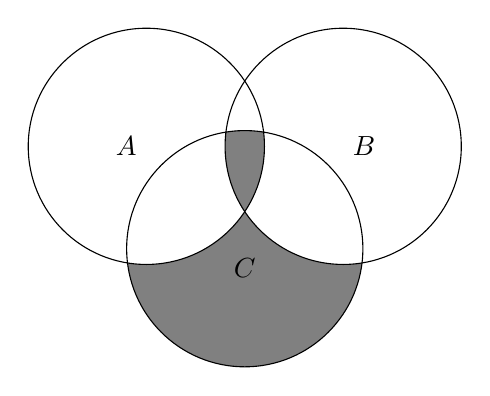
\begin{tikzpicture}
% Define circles for A, B, and C
\def\circleA{(-0.5,0) circle (1.5cm)}
\def\circleB{(2.0,0) circle (1.5cm)}
\def\circleC{(0.75,-1.3) circle (1.5cm)}

% Shade exclusively C (C not A, not B)
\begin{scope}
\clip \circleC;
\fill[gray] \circleC;
\begin{scope}
\clip \circleA;
\fill[white] \circleC;
\end{scope}
\begin{scope}
\clip \circleB;
\fill[white] \circleC;
\end{scope}
\end{scope}

% Shade the intersection of A, B, and C
\begin{scope}
\clip \circleA;
\clip \circleB;
\clip \circleC;
\fill[gray] \circleC;  % fill the intersection with the same color
\end{scope}

% Outline the circles and label them
\draw \circleA node [text=black, left] {$A$};
\draw \circleB node [text=black, right] {$B$};
\draw \circleC node [text=black, below] {$C$};
\end{tikzpicture}
\pagebreak

Below is the prove for \textbf{15(b)}.
\begin{alignat*}{2}
&x \in (A \cap C) \triangle (B \setminus C) && \quad \textbf{(1)}\\
&\equiv x \in [(A \cap C) \setminus (C \setminus B)] \cup [(C \setminus B) \setminus (A \cap C)] && \quad \textbf{(2)}\\
&\equiv x \in [(A \cap C) \setminus (C \setminus B)] \cup Q && \quad \textbf{(3)}\\
&\equiv [x \in (A \cap C) \setminus (C \setminus B)] \vee x \in Q && \quad \textbf{(4)}\\
&\equiv [(x \in A \wedge x \in C) \wedge \neg (x \in C \wedge \neg (x \in B))] \vee x \in Q && \quad \textbf{(5)}\\
&\equiv [(x \in A \wedge x \in C) \wedge (\neg (x \in C) \vee x \in B)] \vee x \in Q && \quad \textbf{(6)}\\
&\equiv \{[(x \in A \wedge x \in C) \wedge \neg (x \in C)] \vee [(x \in A \wedge x \in C) \wedge x \in B]\} \vee x \in Q && \quad \textbf{(7)}\\
&\equiv \{[x \in A \wedge (x \in C \wedge \neg (x \in C))] \vee [(x \in A \wedge x \in C) \wedge x \in B]\} \vee x \in Q && \quad \textbf{(8)}\\
&\equiv \{[x \in A \wedge \text{Contradiction}] \vee [(x \in A \wedge x \in C) \wedge x \in B]\} \vee x \in Q && \quad \textbf{(9)}\\
&\equiv \{\text{Contradiction} \vee [(x \in A \wedge x \in C) \wedge x \in B]\} \vee x \in Q && \quad \textbf{(10)}\\
&\equiv [(x \in A \wedge x \in C) \wedge x \in B] \vee x \in Q && \quad \textbf{(11)}\\
&\equiv [x \in A \wedge x \in C \wedge x \in B] \vee x \in Q && \quad \textbf{(12)}\\
&\equiv [x \in C \wedge (x \in A \wedge x \in B)] \vee x \in Q && \quad \textbf{(13)}\\
&\equiv x \in P \vee x \in Q && \quad \textbf{(14)}\\
&\equiv x \in P \vee [x \in (C \setminus B) \setminus (A \cap C)] && \quad \textbf{(15)}\\
&\equiv x \in P \vee \{(x \in C \wedge \neg (x \in B)) \wedge \neg (x \in A \wedge x \in C)\} && \quad \textbf{(16)}\\
&\equiv x \in P \vee \{(x \in C \wedge \neg ( x \in B)) \wedge (\neg (x \in A) \vee \neg (x \in C))\} && \quad \textbf{(17)}\\
&\equiv x \in P \vee \{[(x \in C \wedge \neg (x \in B)) \wedge \neg (x \in A)] \vee [(x \in C) \wedge \neg (x \in B)) \wedge \neg (x \in C)]\} && \quad \textbf{(18)}\\
&\equiv x \in P \vee \{[(x \in C \wedge \neg (x \in B)) \wedge \neg (x \in A)] \vee [(x \in C \wedge \neg (x \in C)) \wedge \neg (x \in B)]\} && \quad \textbf{(19)}\\
&\equiv x \in P \vee \{[(C \wedge \neg B) \wedge \neg A] \vee [\text{Contradiction} \wedge \neg B]\} && \quad \textbf{(20)}\\
&\equiv x \in P \vee \{[(x \in C \wedge \neg (x \in B)) \wedge \neg (x \in A)] \vee \text{Contradiction}\} && \quad \textbf{(21)}\\
&\equiv x \in P \vee [(x \in C \wedge \neg (x \in B)) \wedge \neg (x \in A)] && \quad \textbf{(22)}\\
&\equiv x \in P \vee [x \in C \wedge (\neg (x \in B) \wedge \neg (x \in A))] && \quad \textbf{(23)}\\
&\equiv x \in P \vee [x \in C \wedge \neg (x \in A \vee x \in B)] && \quad \textbf{(24)}\\
&\equiv [x \in C \wedge (x \in A \wedge x \in B)] \vee [x \in C \wedge \neg (x \in A \vee x \in B)] && \quad \textbf{(25)}\\
&\equiv x \in C \wedge [(x \in A \wedge x \in B) \vee \neg (x \in A \vee x \in B)] && \quad \textbf{(26)}\\
&\equiv x \in C \wedge [\neg (x \in A \vee x \in B) \vee (x \in A \wedge x \in B)] && \quad \textbf{(27)}\\
&\equiv x \in C \wedge \neg [(x \in A \vee x \in B) \wedge \neg (x \in A \wedge x \in B)] && \quad \textbf{(28)}\\
&\equiv x \in C \wedge \neg [(x \in A \cup B) \wedge \neg (x \in A \cap B)] && \quad \textbf{(29)}\\
&\equiv x \in C \wedge \neg [x \in (A \cup B) \setminus (A \cap B)] && \quad \textbf{(30)}\\
&\equiv x \in C \setminus [(A \cup B) \setminus (A \cap B)] && \quad \textbf{(31)}\\
&\equiv x \in C \setminus (A \triangle B) && \quad \textbf{(32)}\\
&\qed
\end{alignat*}
\pagebreak

Below is the chain of justification corresponding to the proof of \textbf{15(b)}.

\begin{alignat*}{2}
&\textbf{(1)} && \quad \text{RHS} \\
&\textbf{(2)} && \quad \text{Def. of Symmetric Difference} \\
&\textbf{(3)} && \quad \text{Substitution: } Q = [(C \setminus B) \setminus (A \cap C)] \\
&\textbf{(4)} && \quad \text{Def. of Union of Sets} \\
&\textbf{(5)} && \quad \text{Def. of Difference and Intersection of Sets} \\
&\textbf{(6)} && \quad \text{DeMorgan's Law} \\
&\textbf{(7)} && \quad \text{Distributive Law} \\
&\textbf{(8)} && \quad \text{Associative Law} \\
&\textbf{(9)} && \quad \text{Def. of Contradiction} \\
&\textbf{(10)} && \quad \text{Law of Contradiction} \\
&\textbf{(11)} && \quad \text{Law of Contradiction} \\
&\textbf{(12)} && \quad \text{Associative Law} \\
&\textbf{(13)} && \quad \text{Commutative and Associative Law} \\
&\textbf{(14)} && \quad \text{Substitution: } P = [C \cap (A \cap B)] \\
&\textbf{(15)} && \quad \text{Substitution: } Q = [(C \setminus B) \setminus (A \cap C)] \\
&\textbf{(16)} && \quad \text{Def. of Difference and Intersection of Sets} \\
&\textbf{(17)} && \quad \text{DeMorgan's Law} \\
&\textbf{(18)} && \quad \text{Distributive Law} \\
&\textbf{(19)} && \quad \text{Commutative and Associative Law} \\
&\textbf{(20)} && \quad \text{Def. of Contradiction} \\
&\textbf{(21)} && \quad \text{Law of Contradiction} \\
&\textbf{(22)} && \quad \text{Law of Contradiction} \\
&\textbf{(23)} && \quad \text{Associative Law} \\
&\textbf{(24)} && \quad \text{DeMorgan's Law} \\
&\textbf{(25)} && \quad \text{Substitution: } P = [C \cap (A \cap B)] \\
&\textbf{(26)} && \quad \text{Distributive Law} \\
&\textbf{(27)} && \quad \text{Commutative Law} \\
&\textbf{(28)} && \quad \text{DeMorgan's Law} \\
&\textbf{(29)} && \quad \text{Def. of Union and Intersection of Sets} \\
&\textbf{(30)} && \quad \text{Def. of Difference of Sets} \\
&\textbf{(31)} && \quad \text{Def. of Difference of Sets} \\
&\textbf{(32)} && \quad \text{Def. of Symmetric Difference, LHS} \\
\end{alignat*}
\pagebreak

\textbf{15(c)}: Consider that $(B \setminus A) \triangle C \equiv [A \cap B \cap C] \cup [C \cap \neg (A \cup B)]$. \\ The corresponding Venn diagram is shown below. \\
The diagram is drawn by noting that (via diagrams):
$$(B \setminus A) \triangle C \equiv [B \setminus (A \cup C)] \cup [C \setminus (B \setminus A)] \equiv [B \setminus (A \cup C)] \cup (C \setminus B) \cup (C \cap A)$$
Drawing Venn diagrams, and trial and error will reveal that $(B \setminus A) \triangle C = (A \triangle C) \triangle (A \cup B)$.

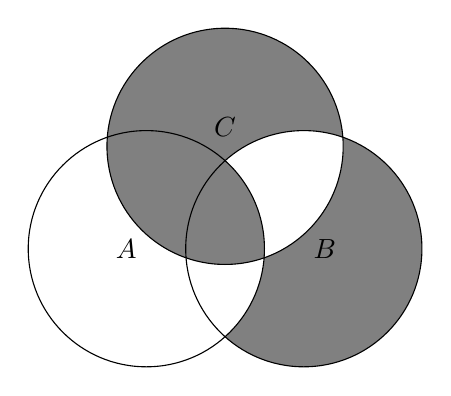
\begin{tikzpicture}
% Define circles for A, B, and C
\def\circleA{(-1,0) circle (1.5cm)}
\def\circleB{(1,0) circle (1.5cm)}
\def\circleC{(0,1.3) circle (1.5cm)}
% Shade B \ (A ∪ C)
\begin{scope}
\clip \circleB;
\fill[gray] \circleB;
\begin{scope}
\clip \circleA;
\fill[white] \circleA;
\end{scope}
\begin{scope}
\clip \circleC;
\fill[white] \circleC;
\end{scope}
\end{scope}
% Shade C \ B
\begin{scope}
\clip \circleC;
\fill[gray] \circleC;
\begin{scope}
\clip \circleB;
\fill[white] \circleB;
\end{scope}
\end{scope}
% Shade C ∩ A
\begin{scope}
\clip \circleC;
\clip \circleA;
\fill[gray] \circleA;
\end{scope}
% Outline the circles and label them
\draw \circleA node [text=black, left] {$A$};
\draw \circleB node [text=black, right] {$B$};
\draw \circleC node [text=black, above] {$C$};
\end{tikzpicture}

Below is the prove for  \textbf{15(c)}.
\begin{alignat*}{2}
x \in (A \triangle C) \triangle (A \cup B) &\equiv x \in A \triangle [C \triangle (A \cup B)] && \quad \textbf{(1)}\\
&\equiv x \in A \triangle [(A \cup B) \triangle C] && \quad \textbf{(2)}\\
&\equiv x \in [A \triangle (A \cup B)] \triangle C && \quad \textbf{(3)}\\
&\equiv x \in [(A \cup B) \triangle A] \triangle C && \quad \textbf{(4)}\\
&\equiv x \in [(A \triangle A) \triangle (B \setminus A)] \triangle C && \quad \textbf{(5)}\\
&\equiv x \in [\emptyset \triangle (B \setminus A)] \triangle C && \quad \textbf{(6)}\\
&\equiv x \in ([\emptyset \cup (B \setminus A)] \setminus [\emptyset \cap (B \setminus A)] ) \triangle C && \quad \textbf{(7)}\\
&\equiv x \in [(B \setminus A) \setminus \emptyset] \triangle C && \quad \textbf{(8)}\\
&\equiv x \in (B \setminus A) \triangle C && \quad \textbf{(9)}\\
\end{alignat*}

Below is the corresponding chain of justification for \textbf{Exercise 15(c)}.
\begin{alignat*}{2}
&\textbf{(1)} && \quad \text{\textbf{Exercise 12} Associative Law, RHS}\\
&\textbf{(2)} && \quad \text{\textbf{Exercise 14(c) Proof Line 3} Commutative Law}\\
&\textbf{(3)} && \quad \text{\textbf{Exercise 12} Associative Law}\\
&\textbf{(4)} && \quad \text{\textbf{Exercise 14(c) Proof Line 3} Commutative Law}\\
&\textbf{(5)} && \quad \text{\textbf{Exercise 14(a)} Result of Exercise}\\
&\textbf{(6)} && \quad A \triangle A \equiv (A \cup A) \setminus (A \cap A) \equiv A \setminus A \equiv \emptyset\\
&\textbf{(7)} && \quad \emptyset \cup X \equiv X \quad \text{and} \quad \emptyset \cap X \equiv \emptyset\\
&\textbf{(8)} && \quad X \setminus \emptyset \equiv X \wedge \neg \emptyset \equiv X \wedge U \equiv X \quad \text{, where $U$ is the universal set and $\neg \emptyset \equiv U$}\\
&\textbf{(9)} && \quad \text{LHS}\\
\end{alignat*}